\addcontentsline{toc}{part}{Chapters}
\chapter{Title of First Chapter}

Some text (\cite{aarts2007}). Some text \textcite{aarts2007}; Some text Aarts (\citeyear{aarts2007}).

Take a look at Figure \ref{fig:sigmoid}.

\begin{figure}
\caption{Relationship between processing difficulty and helpfulness of resumption} \label{fig:sigmoid}
\raggedright\setstretch{1}
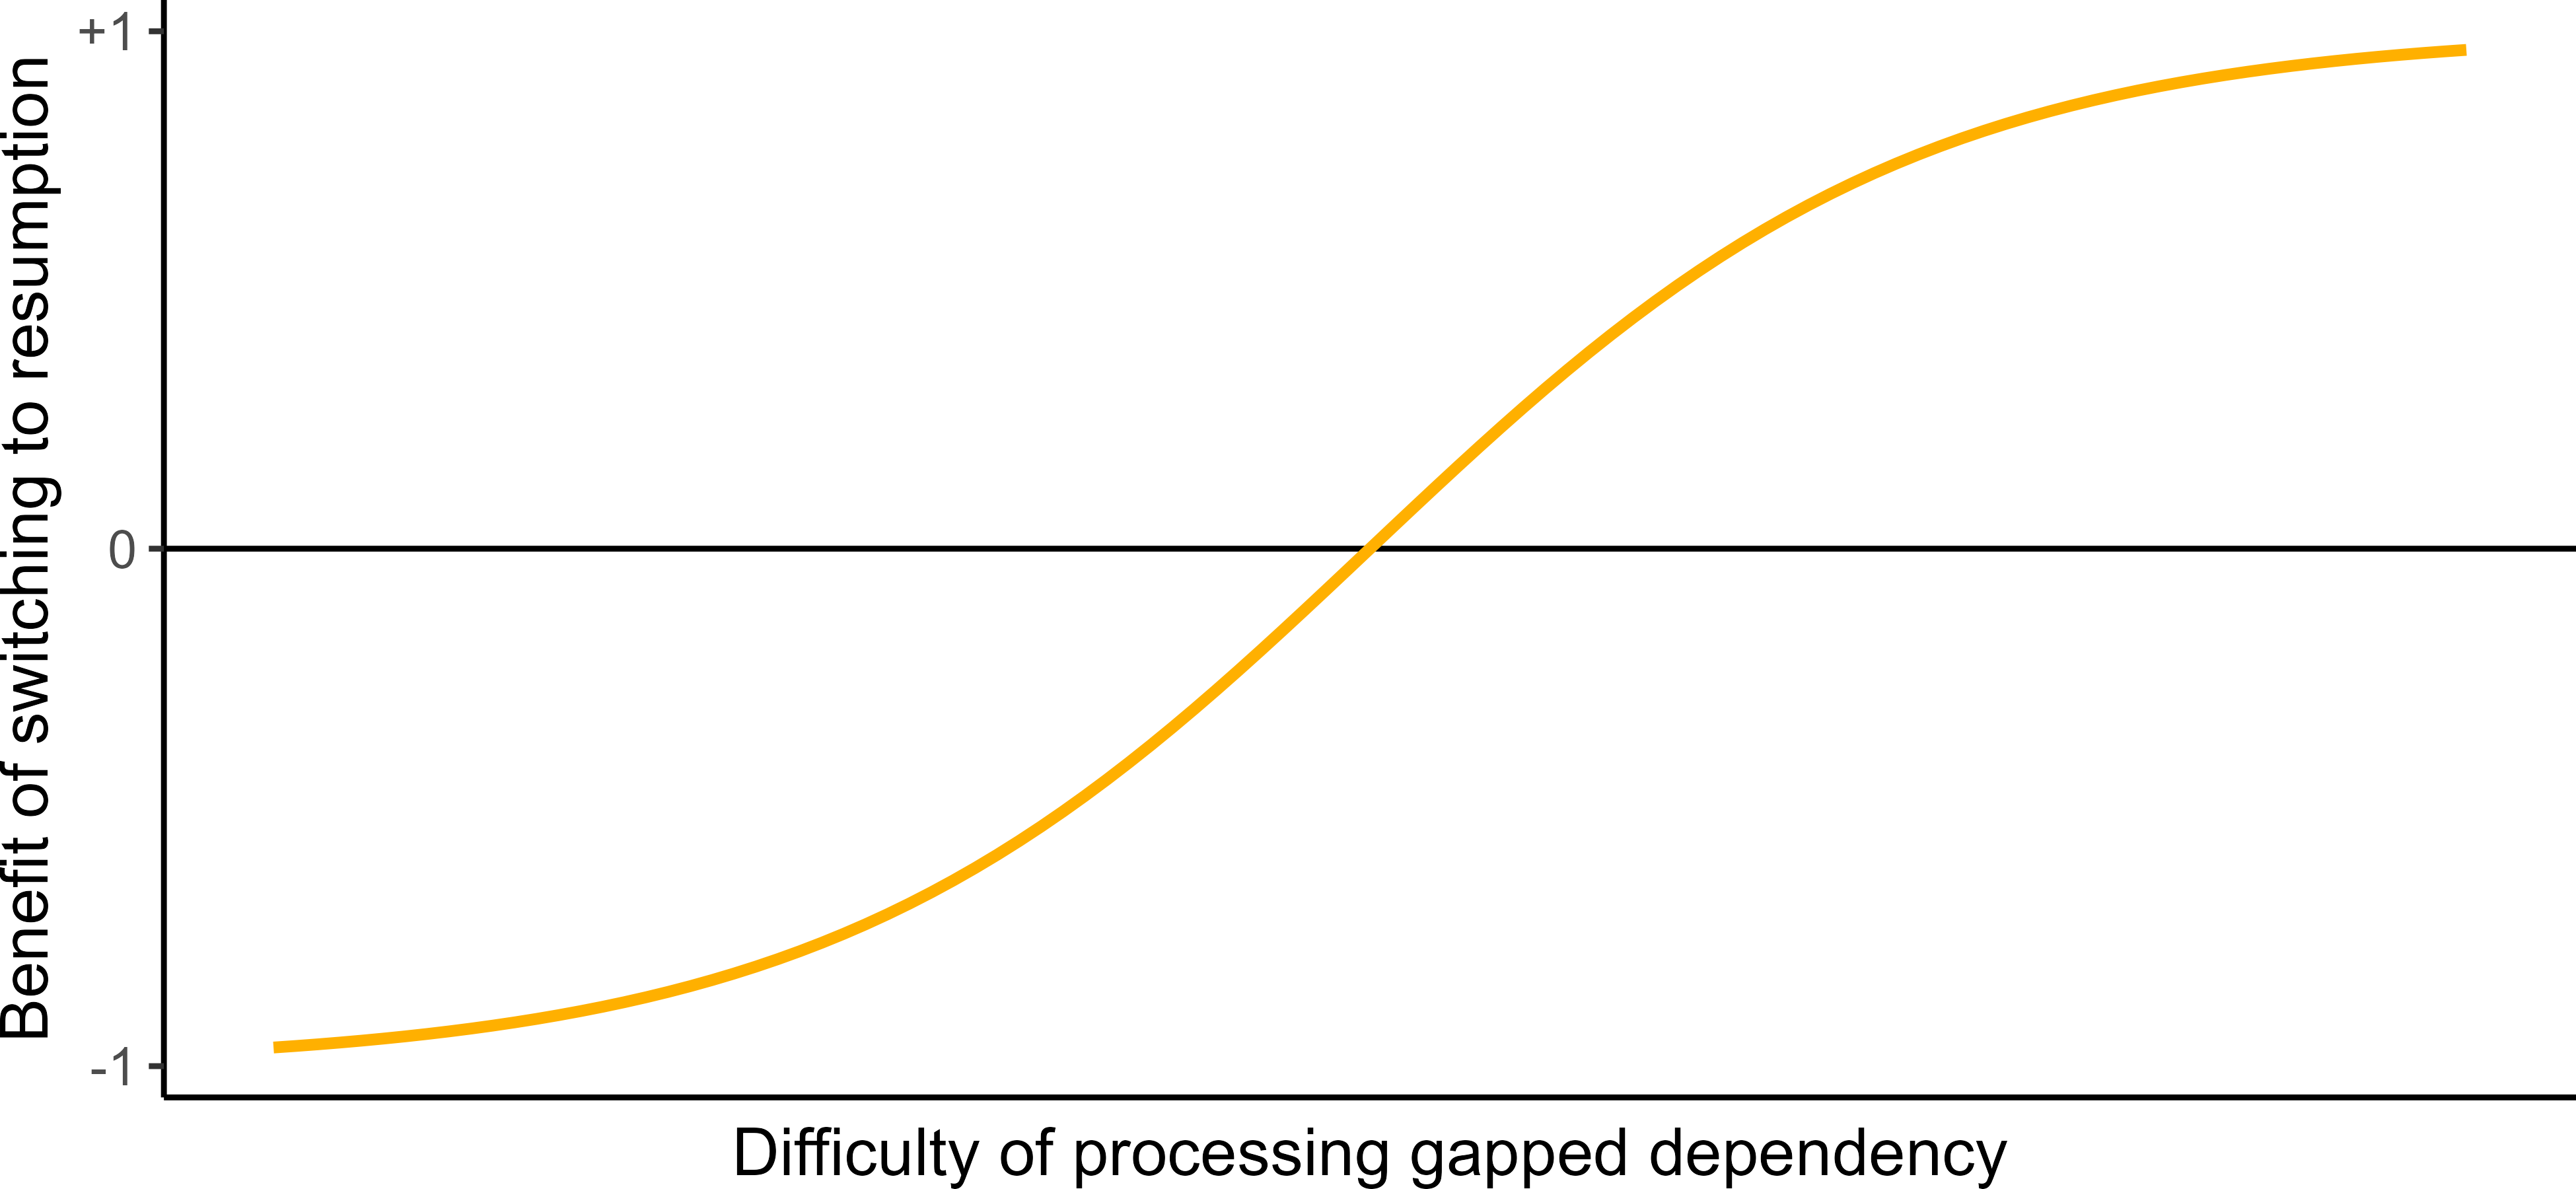
\includegraphics{image/sigmoid.png}
\vspace{-12pt}
\end{figure}

\noindent Some text.

\newpage

Of the four attempts at relativization shown below in Table \ref{tab:constraint}, the one in the [+Aboutness; +Sentential Category] cell (i.e.,~\textit{the dog that is fat}) is the only well-formed RC because it satisfies both the aboutness constraint and the sentential category constraint.

\begin{table}
\caption{Demonstration of the aboutness constraint and the sentential category constraint}\label{tab:constraint}
\raggedright\setstretch{1}
\begin{tabularx}{\linewidth}{XXX}\hline
& \phantom{* }+Aboutness & \phantom{* }−Aboutness\\\hline
+Sentential Category & \phantom{* }the dog [that is fat] & * the dog [that the cat is fat]\\
−Sentential Category & * the dog [that fat] & * the dog [that the cat]\\\hline
\end{tabularx}
\vspace{-12pt}
\end{table}

\noindent Some text.

\ex
people [who like dogs] \label{ex-horse}
\xe

\pex \label{ex-constraint}
\a Aboutness constraint: \par\nobreak\vspace{5pt} RCs are adjuncts and as such must provide supplementary information about their heads.
\a Sentential category constraint: \par\nobreak\vspace{5pt} RCs are sentential categories and as such must consist of at least one predicate and its core arguments, whose presence may be either overtly expressed or merely implied.
\xe

\pex[everygla=\ko] \label{ex-dog-ko}
\a
\begingl
\gla 뚱뚱한 개 //
\glb ttungttungha-n kay //
\glc fat-{\sc adn} dog //
\glft `the fat dog' / `the dog that is fat' //
\endgl \label{ex-dog-ko-1}
\a
\begingl
\gla 고양이를 좋아한 개 //
\glb koyangi-lul cohaha-n kay //
\glc cat-{\sc acc} like-{\sc adn} dog //
\glft `the dog that liked the cat' //
\endgl \label{ex-dog-ko-2}
\xe

\pex[everygla=\zh] \label{ex-dog-zh}
\a
\begingl
\gla 胖 的 狗 //
\glb pang de gou //
\glc fat {\sc adn} dog //
\glft `the fat dog' / `the dog that is fat' //
\endgl \label{ex-dog-zh-1}
\a
\begingl
\gla 喜歡 貓 的 狗 //
\glb xihuan mao de gou //
\glc like cat {\sc adn} dog //
\glft `the dog that likes the cat' //
\endgl \label{ex-dog-zh-2}
\xe